% Options for packages loaded elsewhere
\PassOptionsToPackage{unicode}{hyperref}
\PassOptionsToPackage{hyphens}{url}
%
\documentclass[
  12pt,
]{article}
\usepackage{amsmath,amssymb}
\usepackage{lmodern}
\usepackage{ifxetex,ifluatex}
\ifnum 0\ifxetex 1\fi\ifluatex 1\fi=0 % if pdftex
  \usepackage[T1]{fontenc}
  \usepackage[utf8]{inputenc}
  \usepackage{textcomp} % provide euro and other symbols
\else % if luatex or xetex
  \usepackage{unicode-math}
  \defaultfontfeatures{Scale=MatchLowercase}
  \defaultfontfeatures[\rmfamily]{Ligatures=TeX,Scale=1}
\fi
% Use upquote if available, for straight quotes in verbatim environments
\IfFileExists{upquote.sty}{\usepackage{upquote}}{}
\IfFileExists{microtype.sty}{% use microtype if available
  \usepackage[]{microtype}
  \UseMicrotypeSet[protrusion]{basicmath} % disable protrusion for tt fonts
}{}
\makeatletter
\@ifundefined{KOMAClassName}{% if non-KOMA class
  \IfFileExists{parskip.sty}{%
    \usepackage{parskip}
  }{% else
    \setlength{\parindent}{0pt}
    \setlength{\parskip}{6pt plus 2pt minus 1pt}}
}{% if KOMA class
  \KOMAoptions{parskip=half}}
\makeatother
\usepackage{xcolor}
\IfFileExists{xurl.sty}{\usepackage{xurl}}{} % add URL line breaks if available
\IfFileExists{bookmark.sty}{\usepackage{bookmark}}{\usepackage{hyperref}}
\hypersetup{
  pdftitle={Spatial modeling of K-12 school shootings as a Matern clustered point process},
  pdfauthor={J Steven Raquel},
  hidelinks,
  pdfcreator={LaTeX via pandoc}}
\urlstyle{same} % disable monospaced font for URLs
\usepackage[margin=0.5in]{geometry}
\usepackage{graphicx}
\makeatletter
\def\maxwidth{\ifdim\Gin@nat@width>\linewidth\linewidth\else\Gin@nat@width\fi}
\def\maxheight{\ifdim\Gin@nat@height>\textheight\textheight\else\Gin@nat@height\fi}
\makeatother
% Scale images if necessary, so that they will not overflow the page
% margins by default, and it is still possible to overwrite the defaults
% using explicit options in \includegraphics[width, height, ...]{}
\setkeys{Gin}{width=\maxwidth,height=\maxheight,keepaspectratio}
% Set default figure placement to htbp
\makeatletter
\def\fps@figure{htbp}
\makeatother
\setlength{\emergencystretch}{3em} % prevent overfull lines
\providecommand{\tightlist}{%
  \setlength{\itemsep}{0pt}\setlength{\parskip}{0pt}}
\setcounter{secnumdepth}{5}
\usepackage{setspace}
\usepackage{booktabs}
\usepackage{longtable}
\usepackage{array}
\usepackage{multirow}
\usepackage{wrapfig}
\usepackage{float}
\floatplacement{figure}{H}
\usepackage{subfig}
\usepackage{booktabs}
\usepackage{longtable}
\usepackage{array}
\usepackage{multirow}
\usepackage{wrapfig}
\usepackage{float}
\usepackage{colortbl}
\usepackage{pdflscape}
\usepackage{tabu}
\usepackage{threeparttable}
\usepackage{threeparttablex}
\usepackage[normalem]{ulem}
\usepackage{makecell}
\usepackage{xcolor}
\ifluatex
  \usepackage{selnolig}  % disable illegal ligatures
\fi

\title{Spatial modeling of K-12 school shootings as a Matern clustered
point process}
\usepackage{etoolbox}
\makeatletter
\providecommand{\subtitle}[1]{% add subtitle to \maketitle
  \apptocmd{\@title}{\par {\large #1 \par}}{}{}
}
\makeatother
\subtitle{STATS 295 Winter 2022 Spatial Analysis}
\author{J Steven Raquel}
\date{}

\begin{document}
\maketitle

\hypertarget{introduction}{%
\section{Introduction}\label{introduction}}

The prevalence of gun violence in schools in the United States has been
referred to both as an epidemic and a public health crisis, and one that
has steadily increased over the past several decades. Apart from the
trauma that such an event can bring to a community, there is also
resonant fear that such incidents inspire copycat events on a local and
a larger scale. This spatial analysis attempts to model the incidence of
these shootings as a Poisson point process, in order to ascertain
whether the locations and events occur with complete spatial randomness,
and thereafter create a model with which these events can be predicted.
Ultimately, a Cox Matern cluster process model was decided upon, which
lead us to conclude that school shooting events may in fact give rise to
future school shootings around them.

\hypertarget{methods}{%
\section{Methods}\label{methods}}

\hypertarget{data}{%
\subsection{Data}\label{data}}

The data was sourced directly from the K-12 School Shooting Database
made available by the Center for Homeland Defense and Security, and was
specifically subset to between the years of 1990-2019. The information
that comprises the dataset was determined by a specific process which
entailed asking what exactly comprises a school shooting. Although the
original database contains shootings ruled accidental (from misuse of a
firearm) as well as incidences of gang-related gun violence on school
grounds, among other incidents such as suicide, we did not opt to
consider this data as relevant to this study in particular. Targeted
events related to domestic situations, or the escalation of disputes
(e.g.~fistfights in which one person pulls out a firearm) were also
ruled school shootings for the purposes of this study.

\hypertarget{exploratory-data-analysis}{%
\subsection{Exploratory Data Analysis}\label{exploratory-data-analysis}}

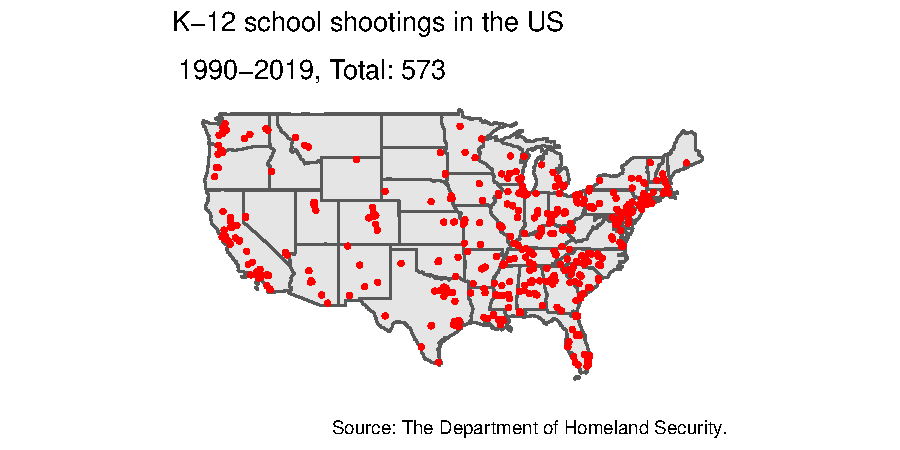
\includegraphics{JStevenRaquel_STATS295_Final_files/figure-latex/plot-point-pattern-9019-1.pdf}

As we can see from the plot above, these events tend to occur in and
around the same places, which gives credence to our hypothesis that the
events exhibit a clustered pattern. We notice in fact, that there are
areas that seem relatively untouched by school shootings in the western
United States, whereas shootings all across the South, Midwest and the
East Coast recur a great deal. While the West Coast is somewhat blighted
by school shootings, particularly in the San Francisco and Los Angeles
metropolitan areas, along with major cities in the Pacific Northwest),
it is not nearly at the rate experienced by the other side of the US.

One thing that it is important to note, as with many spatial analyses
that relate to events caused by humans, that the rate of these events do
correlate in areas with high population density, i.e.~there are more
observations of school shooting events in areas where many people live.
While the implications of this unfortunately will not be well explored
in this literature, it is important to take note of as a confounding
factor when asking questions about the frequency of these events.

\hypertarget{point-pattern-analysis}{%
\subsection{Point Pattern Analysis}\label{point-pattern-analysis}}

With respect to the coordinate-level data, as with any spatial point
pattern analysis, we are concerned with the following three questions,
1) whether the points are located at random, 2) whether they are
clustered, and 3) whether they are placed regularly. Clustering and
regular point patterns respectively are the two opposite ends of the
behavior of a point pattern whereas complete spatial randomness is in
the middle.

The hypothesis of \emph{complete spatial randomness}, or a homogeneous
Poisson process, asserts the following:

\begin{itemize}
\tightlist
\item
  The number of events in any region \(S\) with area \(|S|\) follows a
  Poisson distribution with mean \(\lambda |S|\), where \(\lambda\) is
  the intensity, i.e.~\(\lambda\) does not change over \(S\)
\item
  Given \(n\) events in \(S\), the points \(s_i\) are independently
  located according to the uniform distribution on \(S\), i.e.~there is
  no interaction amongst events.
\end{itemize}

The intensity function \(\lambda(s)\), also known as the first-order
property of the spatial point process, is defined as

\[\lambda(s) = \lim_{|\Delta s| \to 0} \frac{E[N(\Delta s)]}{| \Delta s|}\]

In a homogeneous Poisson process the distribution of events is scattered
all throughout the space such that there are no clusters anywhere nor
any consistent pattern (an example can be seen in the Appendix). We want
to test formally that the data does not follow such a distribution. We
can do this visually first by mapping the density of the data across the
spatial domain.

\hypertarget{kernel-density}{%
\subsubsection{Kernel Density}\label{kernel-density}}

We can visually ascertain as to whether the point pattern \(X\) is
homogeneous by looking at the plot of the Gaussian kernel smoothed
intensity function, which appears as a heatmap. Density based mesasures
look at the first order property of the process, the intensity function,
which illustrates how observations vary from place to place due to the
underlying property, whereas the second order property illustrates how
observations vary from place to place due to interaction effects between
observations themselves (Gimond).

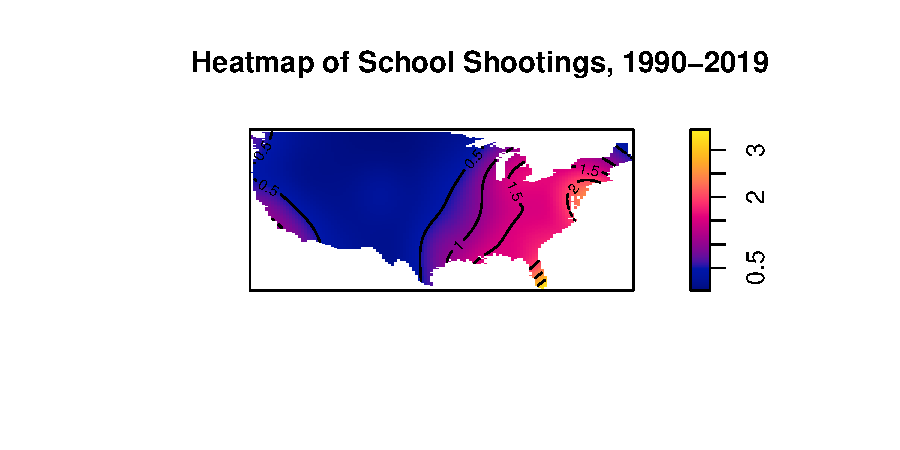
\includegraphics{JStevenRaquel_STATS295_Final_files/figure-latex/density-90-19-1.pdf}

Based on this heatmap of the density function, we note that clustering
is most strong around the south, namely Florida, as well as in the
northeastern United States around New York, where the density is at
least 2. Conversely the density on the west coast is much lower at
around 0.5 along the California coast and the Pacific Northwest. The
center of the US however, is relatively untouched by these events
according to this map.

\hypertarget{quadrats}{%
\subsubsection{Quadrats}\label{quadrats}}

What we are interested in this particular analysis is to how the
intensity varies across different regions contained therein. We do this
by splitting up the area into what are referred to as \emph{quadrats},
small subsets of the event space, and counting the number of events
contained within each quadrat. We can test against the hypothesis of
complete spatial randomness by generating a \(\chi^2\) test statistic
based on the number of expected vs observed events in each quadrat. The
quadrat plot of this process can be seen in the Appendix.

It's important to note the count of events contained within each quadrat
is dependent on the definition of these dimensions, so they can be
subject to misleading conclusions as a result. Since the continental
United States is not shaped like a simple polygon, dividing it into a
reasonable number of equitable and reasonably defined quadrats is not an
easy task and this is a shortcoming we have to recognize.

One methodology for testing for clustering is a Monte Carlo quadrat test
in which we take a number of simulations of patterns under the null
hypothesis e.g.~the homogeneous Poisson point pattern we observed, and
compute a Pearson's \(\chi^2\) test statistic based on the expected and
observed counts in each quadrat, and their residuals. The alternative
hypothesis varies depending on the test, but we want to determine
specifically whether 1) the pattern is homogeneous or not and 2) whether
the pattern is clustered.

The \(\chi^2\) test statistic is given as follows

\[\chi^2 = \sum_{i=1}^n \frac{(O_i - E_i)^2}{E_i}\]

where \(O_i\) is the number of observed events, \(E_i\) is the number of
expected events under the null hypothesis \(H_0\) of complete spatial
randomness, and \(n\) is the total number of events.

\begin{table}[!h]

\caption{\label{tab:tbl-quadrat-test}The results of the quadrat tests of the point process.}
\centering
\resizebox{\linewidth}{!}{
\begin{tabular}[t]{llrrl}
\toprule
Null hypothesis & Alternative hypothesis & Test Statistic & p-Value & Conclusion\\
\midrule
\cellcolor{gray!6}{X is a homogeneous Poisson process} & \cellcolor{gray!6}{X is not a homogeneous Poisson process} & \cellcolor{gray!6}{582.1008} & \cellcolor{gray!6}{4e-04} & \cellcolor{gray!6}{reject H0}\\
X is a homogeneous Poisson process & X is a clustered point pattern & 582.1008 & 2e-04 & reject H0\\
\bottomrule
\end{tabular}}
\end{table}

Based on this table, we have the results of two separate quadrat tests
for our point pattern \(X\), with the null hypothesis of complete
spatial randomness against the corresponding alternative hypotheses of
1) \(X\) not being a homogeneous Poisson process and 2) \(X\) being a
clustered point pattern.

In both cases, our test returns a corresponding p-value of approximately
zero, so we have evidence to reject \(H_0\) in both cases and conclude
that we have respectively in \(X\) not only an inhomogeneous Poisson
process but a clustered point pattern as well. We can further illustrate
this via Ripley's K-function, or more specifically, a transformation of
it.

\hypertarget{ripleys-k-function-and-the-g-function}{%
\subsubsection{Ripley's K-function and the
G-function}\label{ripleys-k-function-and-the-g-function}}

Ripley's K-function of a point process is defined so that
\(\lambda K(r)\) equals the expected number of additional random points
within a distance \(r\) of a typical random point of the point process
\(X\), and is determined by the second order moment properties of \(X\).
Deviations between the empirical and theoretical K-function give us
evidence of spatial clustering or regularity.

\[K(r) = \pi r ^2\]

There are various transformations of the K-function, for example the
L-function proposed by Julian Besag, which stabilizes the variance, or
the G-function, which is the cumulative distribution function of the
distance from a typical random point of \(X\) to the nearest other point
of \(X\), which is particularly effective in diagnosing clustering
behavior in a point process.

The G-function is given by

\[G(r) = 1 - \exp(-\lambda  \pi r^2) = 1 - \exp(-\lambda K(r))\]

We can generate an ``envelope'' of simulated G-functions based on a
spatially random Poisson point pattern, and compare our empirical
G-function from the data to ascertain whether the point pattern \(X\)
has complete spatial randomness or if it is clustered.

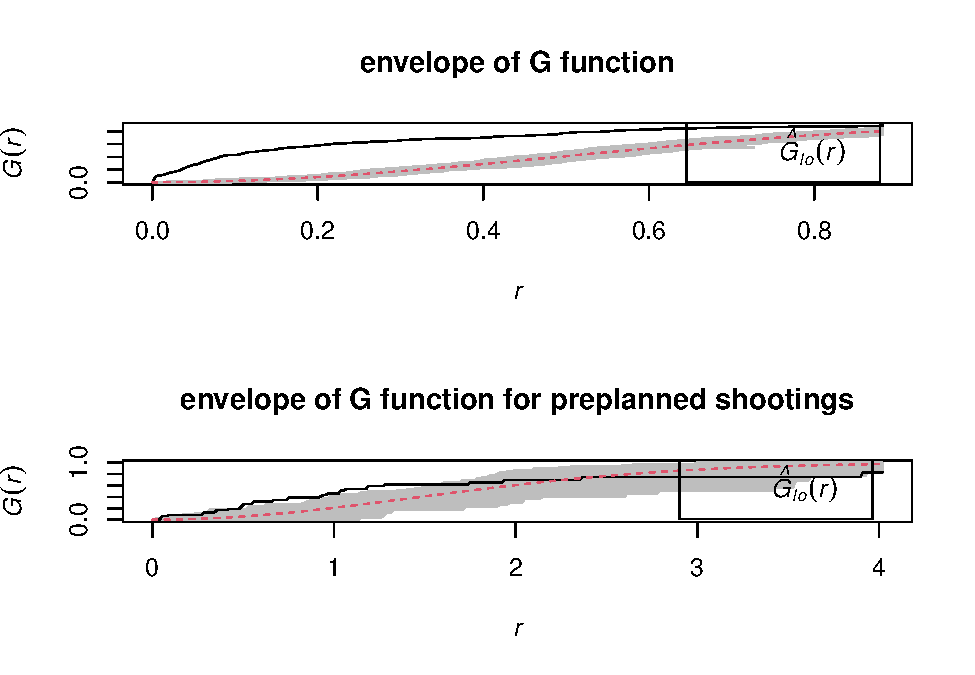
\includegraphics{JStevenRaquel_STATS295_Final_files/figure-latex/plot-G-function-1.pdf}

Contained in this figure we do see a marked difference between the
empirical G-function exceeds the theoretical G-function up to
approximately \(r = 1\), after which point it crosses the envelope of
the point process which exhibits CSR and emerges underneath it. This
does give us evidence that the underlying point process is clustered,
which agrees with the earlier conclusion of our quadrat test.

\hypertarget{modeling}{%
\subsection{Modeling}\label{modeling}}

\hypertarget{the-inhomogeneous-poisson-point-process}{%
\subsubsection{The inhomogeneous Poisson point
process}\label{the-inhomogeneous-poisson-point-process}}

Given that we have confirmed via the quadrat tests and G-function that
the Poisson process is inhomogeneous as well as clustered, our goal at
this point is to develop a model with which we can estimate the
intensity function \(\lambda(s)\).

There are two different methods that we can model this clustered
process: the first, the inhomogeneous Poisson process, assumes that the
process varies spatially as a function of certain covariates, and
assumes that the events themselves are independent. In this context an
inhomogeneous Poisson process assumes that the rate of school shootings
(independently) varies across the spatial domain, which is the
continental United States.

The second method, the Cox process, which is itself a generalization of
the inhomogeneous Poisson process, treats the intensity function
\(\lambda(s)\) itself as a stochastic process that we can model in the
same manner as the first method. The latter also assumes that the events
are not independent of each other. A more benign example of such a
process might be the growth of a forest, since trees leave seeds around
them which then can grow into even more trees. In this context, a Cox
process model assumes that one school shooting event can create even
more.

For an inhomogeneous Poisson process, given the number of events
\(N(B)\) in a subset \(B\) of the spatial domain \(S\), the likelihood
of an inhomogeneous point process is given by

\[P(N(B) = n) \Pi^n_{i=1} P(x_i = s_i) = \frac{1}{n!} \exp(- \int_B \lambda(s) ds) \Pi^n_{i=1} \lambda(s_i)\]

and the log-likelihood is proportional to

\[\log(\lambda(s))= \sum_{j=1}^p \beta_j x_j(s)\]

We can then model the intensity function as

\[\log (\lambda(s)) = \sum_{j=1}^p \beta_j x_j(s)\]

where \(x_j(s), j = 1,...p\) are \(p\) covariates, such that the
log-likelihood is a function of the parameter coefficients \(\beta_j\).

We fit a clustered inhomogeneous Poisson point process model, using the
Matern cluster algorithm. We do not use any other covariates other than
the coordinates in this model. We can use the same methodology of a
quadrat test as we enacted earlier to test the model's appropriateness,
except this time the model under the null hypothesis \(H_0\) follows
that of the estimated intensity function \(\lambda(s)\) of our fitted
model, rather than that of a homogeneous Poisson process. Our
alternative hypothesis \(H_A\) is that the true underlying pattern is
more clustered than that of the null model. Once can refer to the
Appendix for a plot of the envelope of the K-function of this null model
which illustrates this point.

\begin{table}[!h]

\caption{\label{tab:fit2-quadrat-test}Results of the quadrat test for the fitted inhomogenous Poisson process model}
\centering
\resizebox{\linewidth}{!}{
\begin{tabular}[t]{ll}
\toprule
\cellcolor{gray!6}{H0} & \cellcolor{gray!6}{The pattern is explained by the intensity function of the fitted model.}\\
HA & The pattern is more clustered than that explained by the intensity function of the fitted model.\\
\cellcolor{gray!6}{Test Statistic} & \cellcolor{gray!6}{228.805010663107}\\
p-Value & 5e-04\\
\cellcolor{gray!6}{Conclusion} & \cellcolor{gray!6}{reject H0}\\
\bottomrule
\end{tabular}}
\end{table}

With a \(\chi^2\) test-statistic of \(228.81\), we have a p-value of
\(0.001\) which gives us sufficient evidence to reject the fitted
inhomogeneous Poisson process model under the null hypothesis, and
conclude that the true underlying Poisson process is even more clustered
than that of this model.

Having ruled this model out, we want to move on to the Cox point process
model, more specifically, the Matern cluster point process.

\hypertarget{cox-processes-and-the-matern-cluster-process-model}{%
\subsubsection{Cox processes and the Matern cluster process
model}\label{cox-processes-and-the-matern-cluster-process-model}}

Cox process models treat the intensity function \(\lambda(s)\) as a
stochastic process, adding a significant layer of complexity (and
flexibility) relative to the somewhat inflexible inhomogeneous Poisson
process model. More specifically we will be discussing the Matern
cluster process model.

The Matern cluster point process is formed by taking a pattern of
``parent'' points, generated according to some Poisson process with
intensity parameter \(\kappa\), and then generating around it a random
number of ``offspring'' which is itself a Poisson random variable with
mean \(\mu\). The locations of the offspring are independent and
identically distributed via a Uniform distribution in a radius around
the parent defined by the parameter \(R\), also known as the scale.

Our goal is to minimize the discrepancy between the estimated model and
the data, given some constraints. This discrepancy criterion
\(D(\theta)\) is given by

\[D(\theta) = \int_0^{r_0} w(t)[(\hat K(t))^c - (K(t;\theta))^c]^2 dt\]

where we have some parameters \(r_0\), \(c\), and the weight function
\(w(r)\). Minimizing this function is known as the method of minimum
contrast.

It works by first computing the K function, and then deriving the
theoretical expected K value under the point process model. The model is
then fit by tuning the optimal parameter values which minimizes the
difference between the theoretical and empirical K-functions.

The theoretical K-function of this process is given by

\[K(r) = \pi r^2 + \frac{h\large(\frac{r}{2R}\large)}{\kappa}\]

and the theoretical intensity of the process is
\(\lambda = \kappa \mu\).

Recall that earlier we fit an inhomogeneous Poisson point process model
using the Matern cluster algorithm to define the clusters. The model
that was fit returned estimates for not only the intensity function
\(\lambda(s)\), but also \(\kappa\) and \(\mu\), the intensity parameter
of the parent points' pattern, and the mean parameter for the Poisson
random variable of the number of offspring. For values of \(c\) and
\(w(t)\), we want to opt for \(c=0.25\) and a weight function of
\(w(t) = 1\), as these are well suited to well-clustered data.

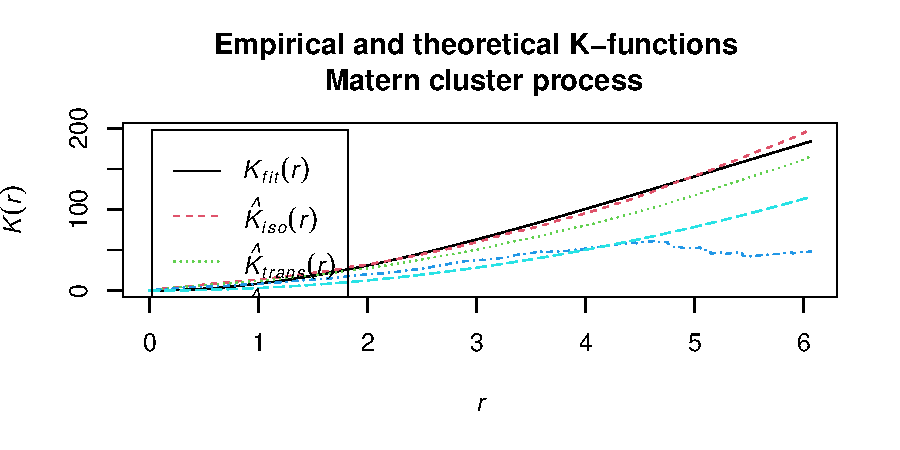
\includegraphics{JStevenRaquel_STATS295_Final_files/figure-latex/plot-matern-process-1.pdf}

This figure gives the theoretical and empirical K-functions of the
Matern cluster process model. The cyan line is the homogeneous Poisson
process, which we have long since established is ill-fitted to the data.
The black line is our empirical K-function, and the red line is the
theoretical K-function under the model.

Based off of this plot of the K-function, it appears in fact that the
Matern cluster process model fit using the intensity and parameter
estimates from the inhomogeneous Poisson process model fit earlier is
fairly consistent at estimating the true underlying process given that
the discrepancy between the theoretical and empirical K-functions is
very low even up to very large distances.

\hypertarget{results}{%
\section{Results}\label{results}}

It's been debated at length as to whether incidences of school shootings
give rise to future events, as long as they've been happening in the
modern day. With respect to how this model applies in context, we have
established that it's indeed possible that this is the case, as
demonstrated by how well the proposed Matern process model fits to the
empirical process. Ascertaining the reason as to why this happens would
have to be left for some future work, perhaps incorporating some of the
unused categorical variables that were included in the data, such as
whether the event was preplanned. The data can also be looked at on an
areal level and compared next to the accessibility of both mental
healthcare and guns (as shown in the Appendix). This was considered as
an initial objective, but was later sidelined in favor of focusing on
analysis of the clustering process. One also wonders how one might model
these tragedies from a spatiotemporal perspective, as it is well
documented how events have been on the rise in the past several years
(also shown in the Appendix).

\begin{table}

\caption{\label{tab:tbl-matern-process}Parameter values chosen for the Matern cluster model.}
\centering
\begin{tabular}[t]{rrrr}
\toprule
kappa & R & c & w(t)\\
\midrule
\cellcolor{gray!6}{0.0172795} & \cellcolor{gray!6}{1.322571} & \cellcolor{gray!6}{0.25} & \cellcolor{gray!6}{1}\\
\bottomrule
\end{tabular}
\end{table}

\hypertarget{conclusion}{%
\subsection{Conclusion}\label{conclusion}}

This Matern cluster process model should be seen first and foremost as a
building block upon which future work by individuals in public health,
sociology, criminology, etc. can build. As with any instances of
tragedy, many unresolved questions remain. Our hope is that some level
of positive inspiration can happen from studying these events such that
we can become better equipped at averting and dealing with these
tragedies.

\newpage

\hypertarget{references}{%
\section{References}\label{references}}

Adrian Baddeley, Ege Rubak, Rolf Turner (2015). Spatial Point Patterns:
Methodology and Applications with R. London: Chapman and Hall/CRC Press,
2015. URL
\url{https://www.routledge.com/Spatial-Point-Patterns-Methodology-and-Applications-with-R/Baddeley-Rubak-Turner/9781482210200/}

Bivand, Roger S. and Wong, David W. S. (2018) Comparing implementations
of global and local indicators of spatial association TEST, 27(3),
716-748. URL \url{https://doi.org/10.1007/s11749-018-0599-x}

Hellebuyck, M., Halpern, M., Nguyen, T. and Fritze, D., 2018. The State
of Mental Health in America. p.9.

Paez A (2021). An Introduction to Spatial Data Analysis and Statistics:
A Course in R. McMaster Invisible Press. ISBN: 978-1-7778515-0-7

Pebesma, E., 2018. Simple Features for R: Standardized Support for
Spatial Vector Data. The R Journal 10 (1), 439-446,
\url{https://doi.org/10.32614/RJ-2018-009}

Riedman, D., Jernegan, E. and O'Neill, D., 2020. K-12 School Shooting
Database. {[}online{]} Center for Homeland Defense and Security.
Available at: \url{https://www.chds.us/ssdb/} {[}Accessed 15 March
2022{]}.

Siegel, M., 2022. State-by-State Firearm Law Data \textbar{} State
Firearm Laws. {[}online{]} Statefirearmlaws.org. Available at:
\url{http://www.statefirearmlaws.org/} {[}Accessed 15 March 2022{]}.

\newpage

\hypertarget{appendix}{%
\section{Appendix}\label{appendix}}

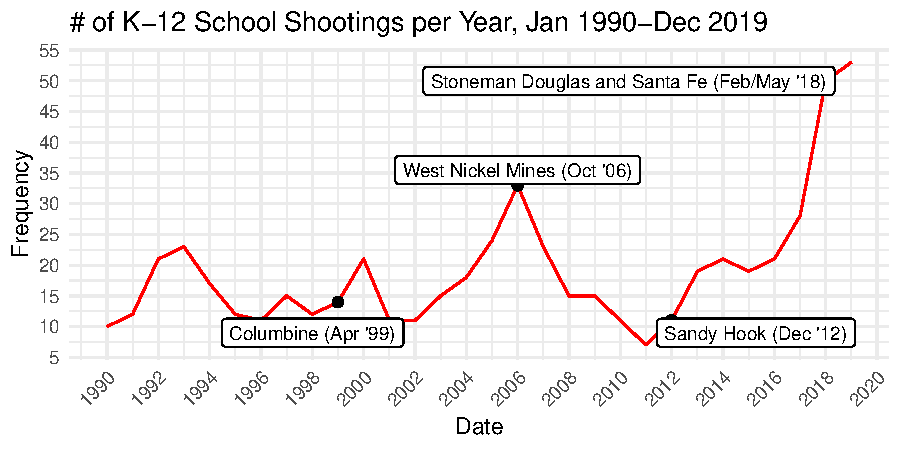
\includegraphics{JStevenRaquel_STATS295_Final_files/figure-latex/ts-plot-1990-2019-1.pdf}

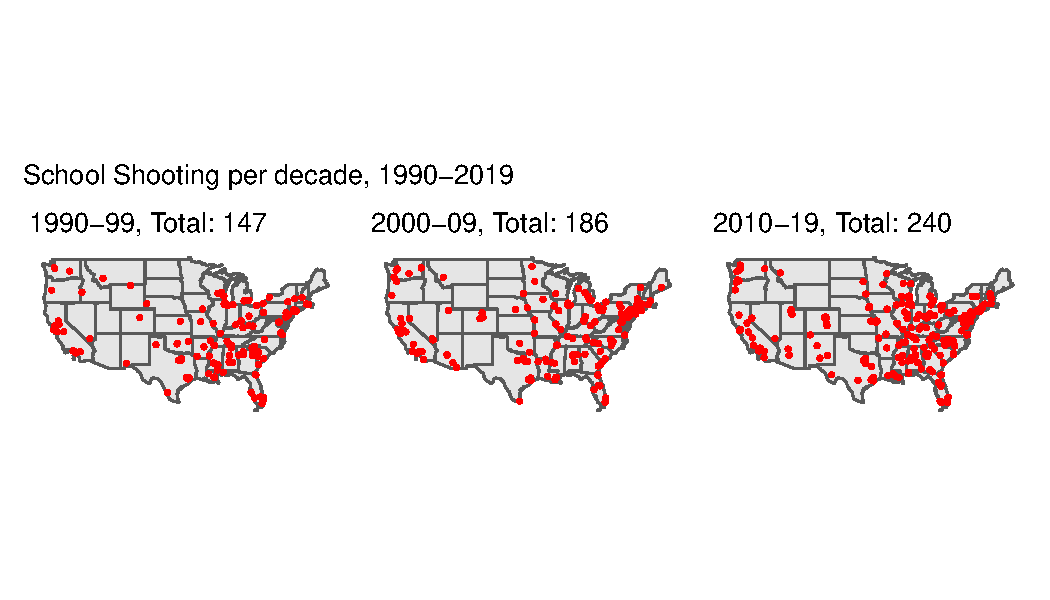
\includegraphics{JStevenRaquel_STATS295_Final_files/figure-latex/plot-point-patterns-1.pdf}

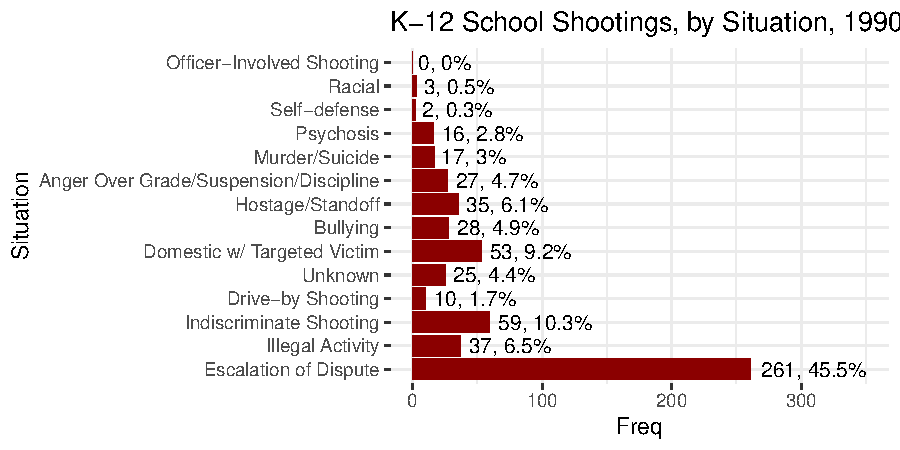
\includegraphics{JStevenRaquel_STATS295_Final_files/figure-latex/plot-situation-1.pdf}

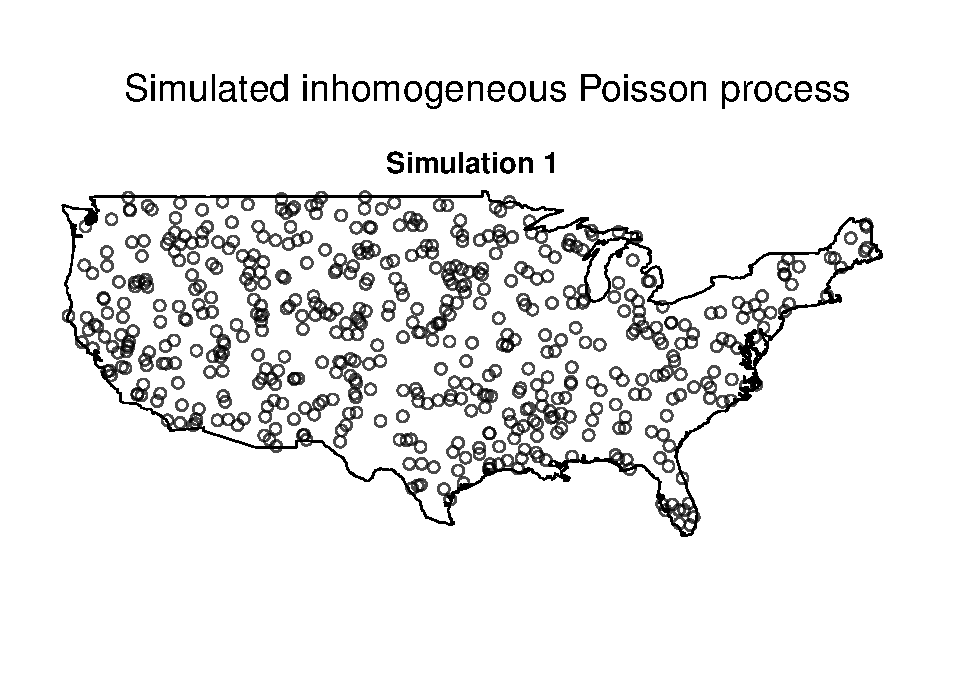
\includegraphics[height=0.75\textheight]{JStevenRaquel_STATS295_Final_files/figure-latex/plot-simulate-ppm-1}

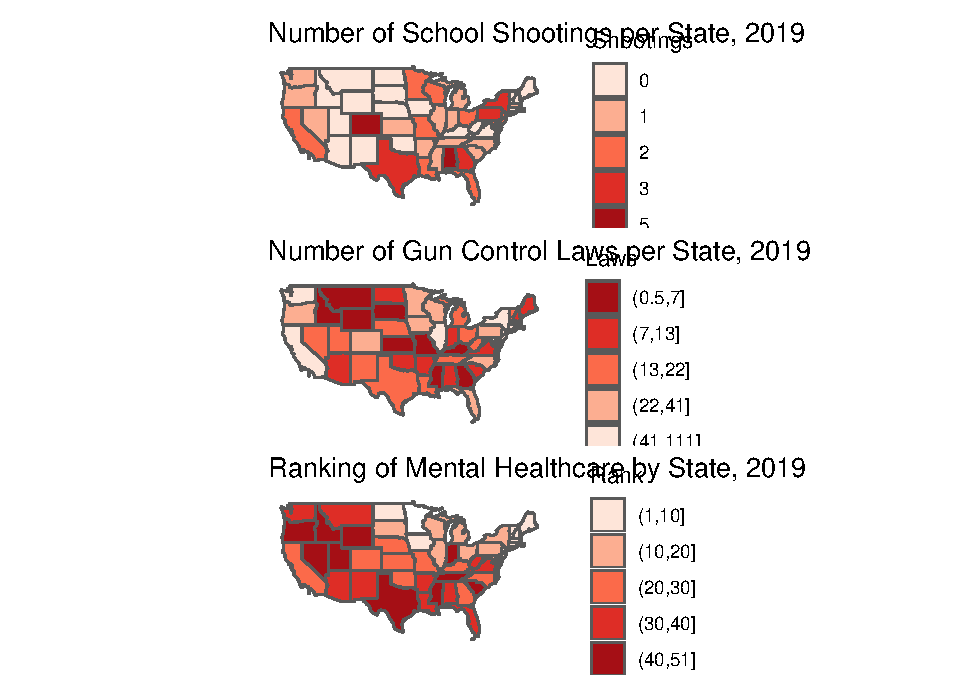
\includegraphics{JStevenRaquel_STATS295_Final_files/figure-latex/plot-areals-2019-1.pdf}
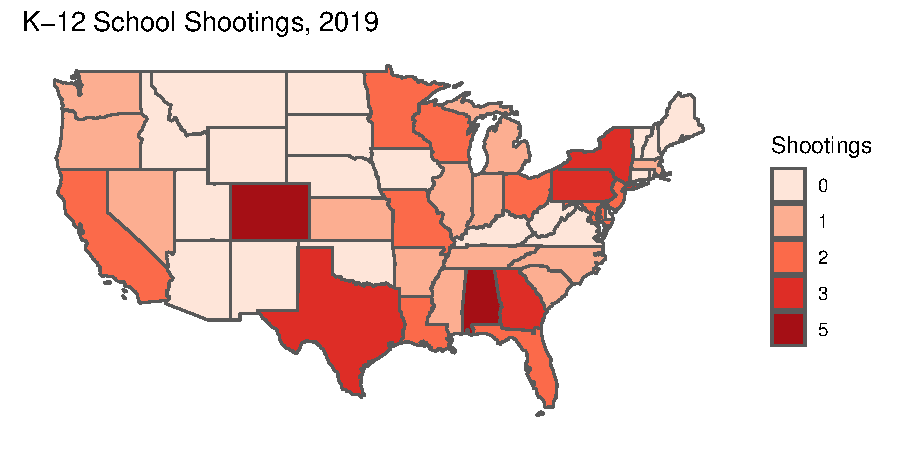
\includegraphics{JStevenRaquel_STATS295_Final_files/figure-latex/plot-areals-2019-2.pdf}
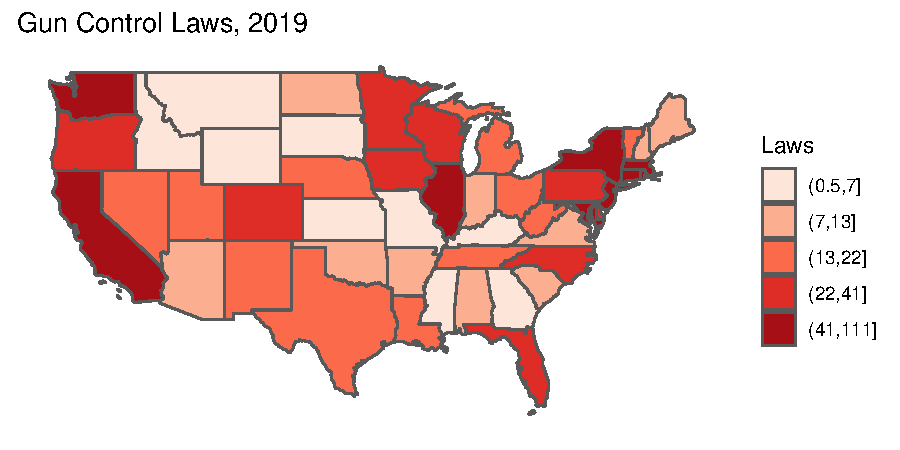
\includegraphics{JStevenRaquel_STATS295_Final_files/figure-latex/plot-areals-2019-3.pdf}
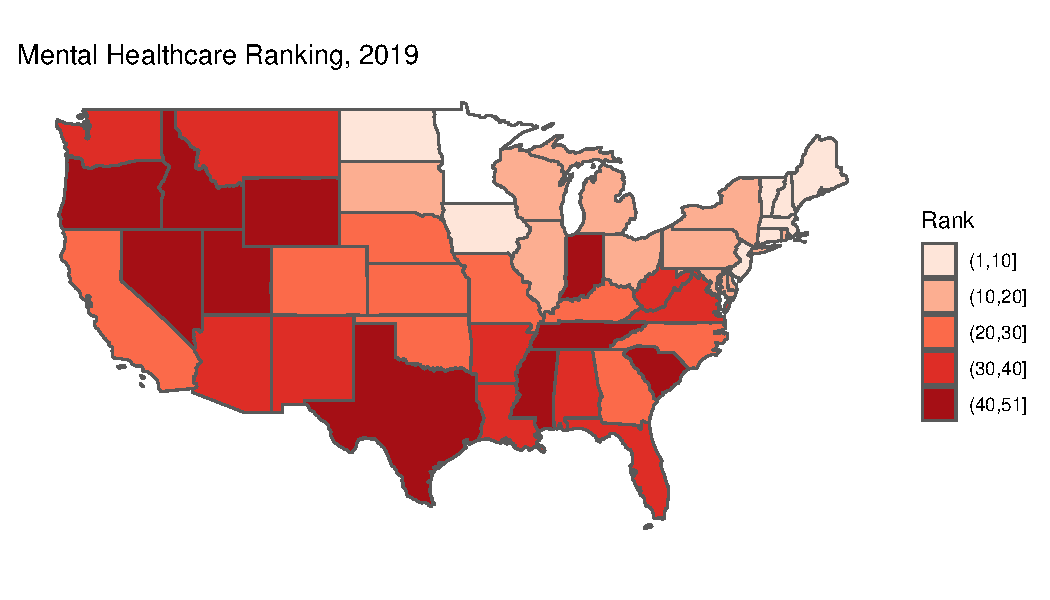
\includegraphics{JStevenRaquel_STATS295_Final_files/figure-latex/plot-areals-2019-4.pdf}

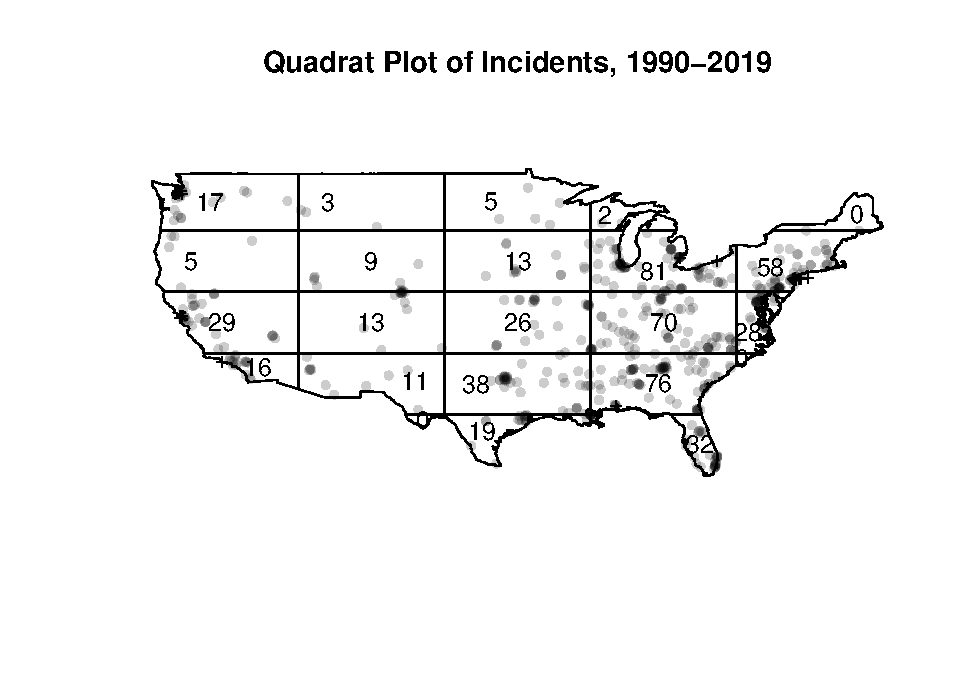
\includegraphics{JStevenRaquel_STATS295_Final_files/figure-latex/plot-quadrats-1990-2019-1.pdf}

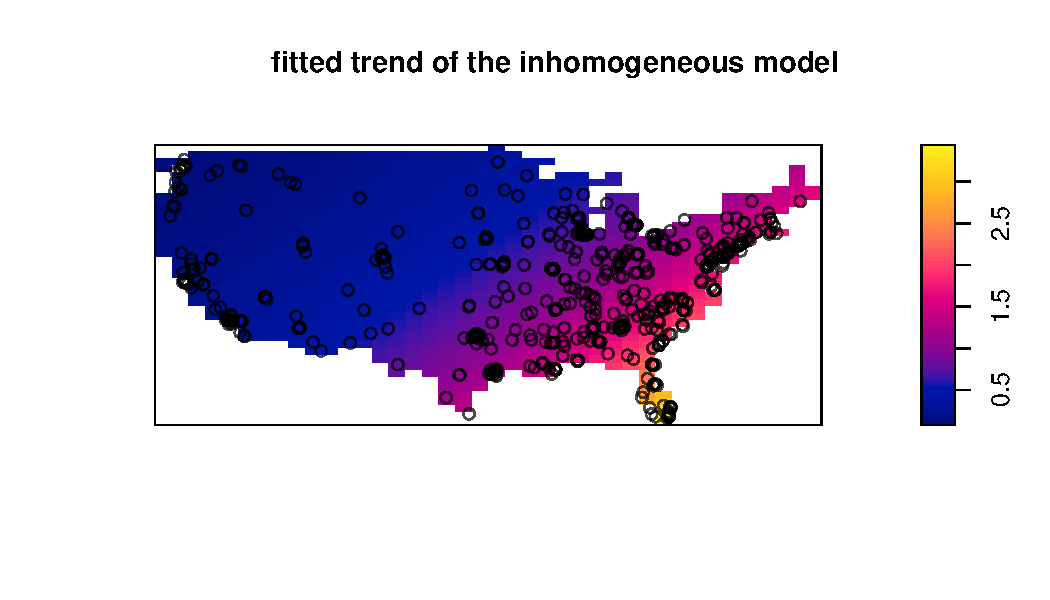
\includegraphics{JStevenRaquel_STATS295_Final_files/figure-latex/plot-fit1-inhomogeneous-1.pdf}

\begin{verbatim}
Conditional Monte Carlo test of fitted Poisson model 'fit1' using
quadrat counts
Test statistic: Pearson X2 statistic
\end{verbatim}

data: data from fit1 X2 = 214.11, = NA, p-value = 5e-04 alternative
hypothesis: clustered

Quadrats: 23 tiles (irregular windows)

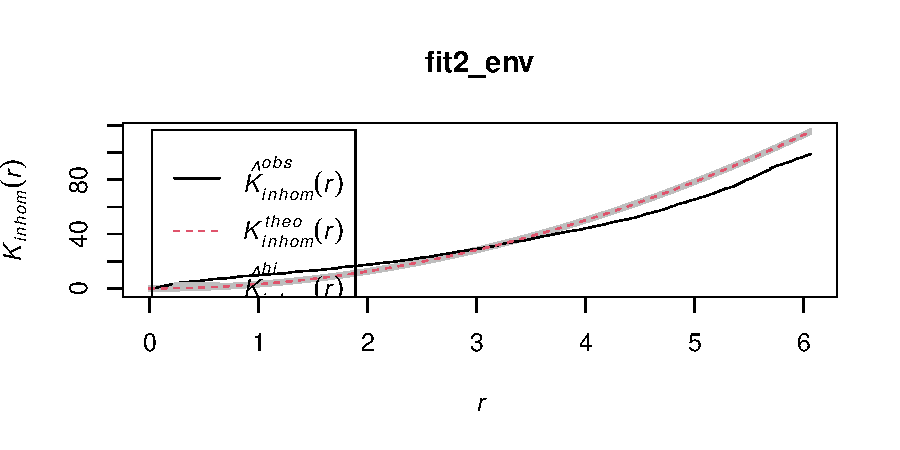
\includegraphics{JStevenRaquel_STATS295_Final_files/figure-latex/plot-fit2-envelope-1.pdf}

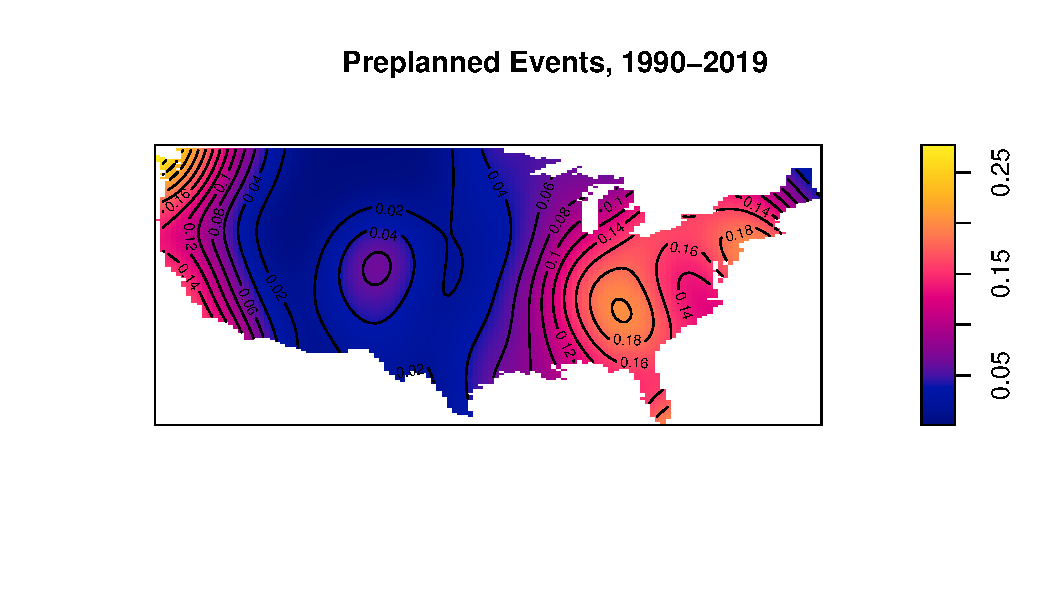
\includegraphics{JStevenRaquel_STATS295_Final_files/figure-latex/heatmap-preplanned-1.pdf}

\end{document}
